\documentclass[11pt,a4paper]{article}

\usepackage[T1]{fontenc}
\usepackage[utf8]{inputenc}
\usepackage{newtxtext,newtxmath}
\usepackage[margin=2.4cm]{geometry}
\usepackage{amsmath}
\usepackage{graphicx}
\usepackage{booktabs}
\usepackage{caption}
\usepackage{subcaption}
\usepackage{enumitem}
\usepackage{microtype}
\usepackage[dvipsnames]{xcolor}
\usepackage[colorlinks=true,linkcolor=NavyBlue,citecolor=NavyBlue,
            urlcolor=NavyBlue]{hyperref}
\usepackage[most]{tcolorbox}
\usepackage{titlesec}

\captionsetup{font=small,labelfont=bf}
\captionsetup[sub]{font=small}
\titleformat{\section}{\large\bfseries}{\thesection}{0.7em}{}
\titleformat{\subsection}{\normalsize\bfseries}{\thesubsection}{0.6em}{}
\setlist{itemsep=1pt,topsep=3pt,parsep=0pt}

\newtcolorbox{keybox}[1]{colback=NavyBlue!5,colframe=NavyBlue!55,
  boxrule=.5pt,arc=2pt,left=6pt,right=6pt,top=4pt,bottom=4pt,
  fonttitle=\bfseries\small,title={#1}}
\newtcolorbox{warnbox}[1]{colback=BrickRed!5,colframe=BrickRed!55,
  boxrule=.5pt,arc=2pt,left=6pt,right=6pt,top=4pt,bottom=4pt,
  fonttitle=\bfseries\small,title={#1}}


\newcommand{\partline}[2]{%
  \bigskip\par\noindent\rule{\textwidth}{0.9pt}\\[3pt]
  {\large\bfseries #1}\hfill{\itshape\small #2}\\[1pt]
  \noindent\rule{\textwidth}{0.35pt}\par\medskip}

\title{\vspace{-1.2cm}\textbf{Unsupervised Learning: Clustering and Anomaly Detection}\\[2pt]
\large A worked summary with illustrations}
\author{Gentian Zavalani}
\date{\small 17 September 2026\\[4pt]
\footnotesize Notes written while working through the Machine Learning
Specialization\\
\footnotesize (DeepLearning.AI, Coursera), Course 3: unsupervised learning}

\begin{document}
\maketitle
\vspace{-0.7cm}

\begin{abstract}\noindent\small
These notes cover the two unsupervised algorithms: $K$-means clustering
(Part~I) and density-estimation anomaly detection (Part~II). Every figure and
every number in the tables was produced by running the algorithms on the
datasets described, not drawn by hand. Each part ends with material the
standard presentation tends to skip. For clustering, that means why the
objective can never choose $K$ for you and why one run of the algorithm is not
enough; for anomaly detection, what the independence assumption costs, what
feature shape costs, and where the arithmetic breaks. In practice these
dominate the outcome.
\end{abstract}

\section{What makes it unsupervised}

Supervised learning is given pairs $(x^{(i)},y^{(i)})$: inputs with the
correct answer attached, from which it learns the map $x \mapsto y$.
Unsupervised learning is given the inputs $x^{(1)},\dots,x^{(m)}$ alone and
must find structure in them. Two tasks:

\begin{itemize}
\item \textbf{Clustering}: partition the data into $K$ groups of similar
      examples. Algorithm: $K$-means.
\item \textbf{Anomaly detection}: learn what \emph{normal} looks like, then
      flag anything that deviates from it.
\end{itemize}

One asymmetry worth noticing immediately. Anomaly detection \emph{trains} on
unlabelled data, but it \emph{tunes} its one free parameter on a small
labelled set. So it is unsupervised in the part that needs lots of data and
supervised in the part that needs almost none. That is exactly the right
split when positive examples are rare and expensive, and it is the reason the
method exists at all.

\partline{Part I\quad Clustering with $K$-means}{find the groups}

\section{The algorithm}

$K$-means partitions the data into $K$ groups by alternating two steps until
the assignments stop changing (Figure~\ref{fig:kmeans}).

\begin{align}
\textbf{assign:}\quad & c^{(i)} := \arg\min_{j\in\{1,\dots,K\}}
  \bigl\| x^{(i)} - \mu_j \bigr\|^2 , \qquad i = 1,\dots,m,
  \label{eq:assign}\\[2pt]
\textbf{move:}\quad & \mu_k := \frac{1}{|C_k|}\sum_{i \in C_k} x^{(i)} ,
  \qquad k = 1,\dots,K ,
  \label{eq:move}
\end{align}

where $C_k = \{\,i : c^{(i)} = k\,\}$ is the set of examples currently assigned
to centroid $k$, and $|C_k|$ is how many there are. The $\mu_k$ are the
\emph{centroids}; $K$ is chosen in advance.

\begin{figure}[t]
\centering
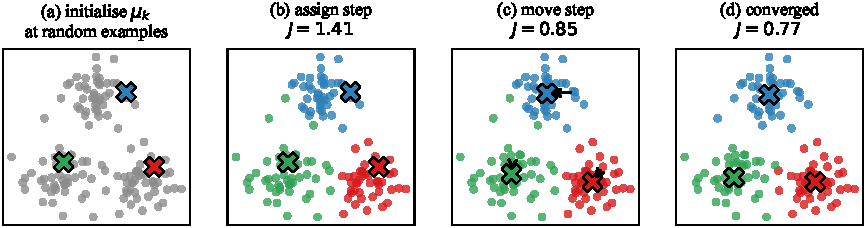
\includegraphics[width=\textwidth]{figs/fig_kmeans.pdf}
\caption{$K$-means on 135 points in three Gaussian blobs, $K=3$. Crosses are
centroids. Panel (b) recolours each point by \eqref{eq:assign}; panel (c)
slides each centroid to the mean of its own colour by \eqref{eq:move}, with
arrows showing the displacement. Both steps decrease the distortion $J$, which
is why the iteration converges. Note that panel (a) initialises the centroids
\emph{at randomly chosen data points}, not at random locations in space.}
\label{fig:kmeans}
\end{figure}

Clustering is used for market segmentation, grouping related news articles,
organising DNA microarray data, grouping astronomical observations, and, as
in Section~\ref{sec:compress}, reducing the number of distinct colours in an
image.

\section{The objective, and why it converges}

Both steps minimise the same quantity, the \emph{distortion}
\begin{equation}
J\bigl(c^{(1)},\dots,c^{(m)},\mu_1,\dots,\mu_K\bigr)
  = \frac{1}{m}\sum_{i=1}^{m} \bigl\| x^{(i)} - \mu_{c^{(i)}} \bigr\|^2 ,
\label{eq:distortion}
\end{equation}
the mean squared distance from each example to the centroid it is assigned to.
The two steps are exactly the two block minimisations of \eqref{eq:distortion}:

\begin{itemize}
\item the \textbf{assign} step minimises $J$ over the $c^{(i)}$ with the
      $\mu_k$ held fixed. For each example independently the best choice is
      the nearest centroid, which is \eqref{eq:assign};
\item the \textbf{move} step minimises $J$ over the $\mu_k$ with the $c^{(i)}$
      held fixed. The minimiser of a sum of squared distances to a set of
      points is their mean, which is \eqref{eq:move}.
\end{itemize}

So $J$ is non-increasing at every half-step. It is bounded below by zero, and
there are only finitely many possible assignments, so the algorithm terminates
in a finite number of iterations. This is coordinate descent, not gradient
descent, and it has no learning rate to tune.

\begin{keybox}{The single most useful debugging check}
$J$ must \textbf{never increase}, not even slightly, at any half-step. If your
implementation shows it rising, you have a bug, almost always a swapped
axis in the distance computation (\texttt{axis=1} where you meant
\texttt{axis=0}) or centroids updated from the previous iteration's
assignments. Print $J$ after every step while developing.
\end{keybox}

\section{Local optima, and why you run it many times}

Termination is guaranteed; \emph{optimality is not}. $K$-means converges to a
local minimum of \eqref{eq:distortion}, and which one depends entirely on the
initialisation. Figure~\ref{fig:localoptima} shows the standard failure: one
true cluster gets split between two centroids while two other clusters are
merged under a third. The result is stable, in the sense that no single
reassignment improves it, and it is more than four times worse than the global
optimum.

\begin{figure}[t]
\centering
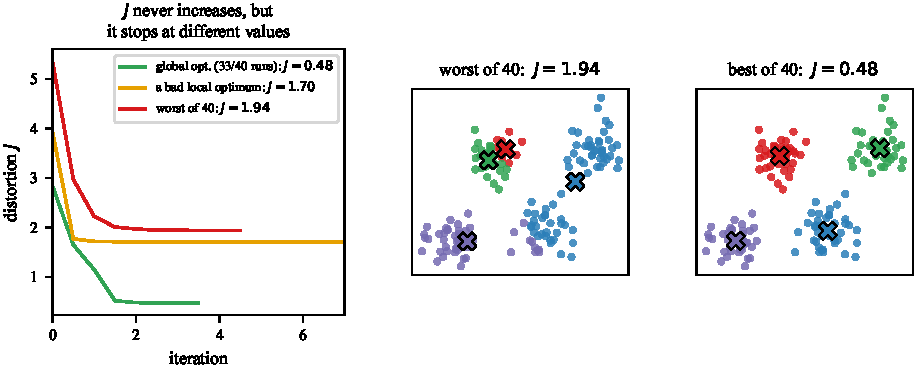
\includegraphics[width=\textwidth]{figs/fig_localoptima.pdf}
\caption{Forty random initialisations on four well-separated clusters. Left:
$J$ against iteration for three of them; every curve is monotone, but they
level off at different values. Middle and right: the worst and best outcomes.
Thirty-three of the forty runs reached $J = 0.48$; the remaining seven got
stuck between $1.70$ and $1.94$. Taking the best of many restarts is not a
refinement, it is a requirement.}
\label{fig:localoptima}
\end{figure}

The fix is to run the whole algorithm many times and keep the best result:

\begin{enumerate}[label=\textbf{\arabic*.}]
\item For $t = 1,\dots,T$ (with $T$ typically $50$ to $1000$):
      initialise $\mu_1,\dots,\mu_K$ at $K$ \emph{randomly chosen distinct
      training examples}, run $K$-means to convergence, and record the final
      $J$.
\item Keep the clustering with the lowest $J$.
\end{enumerate}

Initialising at actual data points matters: it guarantees every centroid
starts somewhere the data actually are, so no cluster is empty at the first
assign step. If a cluster does become empty later, which makes
\eqref{eq:move} a division by zero, either drop that centroid and continue
with $K-1$, or reinitialise it at a random example.

\section{Choosing $K$}

There is no value of $K$ that \eqref{eq:distortion} will pick out for you, and
this is not a gap in the method but a property of the objective: $J$ decreases
monotonically as $K$ grows, reaching zero when $K = m$ and every example is
its own cluster. So $J$ alone can only ever recommend $K = m$.

The \emph{elbow method} plots the best $J$ against $K$ and looks for the point
where the curve stops dropping sharply. Figure~\ref{fig:elbow} shows both why
this is appealing and why it is unreliable. On data with genuine well-separated
clusters there is a sharp elbow at the right $K$. On data that is simply one
elongated blob, which is extremely common, the curve decreases smoothly
and no elbow exists to find. Reporting an elbow from such a curve is reading a
structure into the data that is not there.

\begin{figure}[t]
\centering
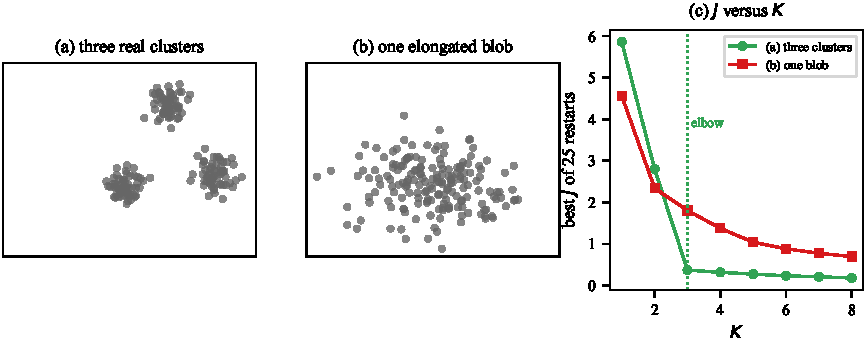
\includegraphics[width=\textwidth]{figs/fig_elbow.pdf}
\caption{The elbow method, and its failure mode. (c) plots the best $J$ over
25 restarts against $K$ for both datasets. The three-cluster data give a sharp
elbow at $K = 3$; the single blob gives a smooth curve with no distinguished
point anywhere.}
\label{fig:elbow}
\end{figure}

The more honest approach is to choose $K$ by what the clusters are \emph{for}.
If you are sizing T-shirts, the question is not which $K$ minimises a sum of
squares but whether the extra manufacturing and inventory cost of five sizes
is repaid by the better fit relative to three. If you are segmenting a market,
$K$ is bounded by how many distinct campaigns you can actually run. Evaluate
$K$ on the downstream objective, not on $J$.

\section{Application: image compression}
\label{sec:compress}

A photograph stores 24 bits per pixel: one byte each for red, green and blue,
so $2^{24} \approx 16.8$ million representable colours. Treat each pixel as a
point $x^{(i)} \in [0,1]^3$ and run $K$-means with $K = 16$ on those points.
The 16 centroids are the 16 colours that best represent the image in the
least-squares sense of \eqref{eq:distortion}, and each pixel is then stored as
the 4-bit index of its nearest centroid (Figure~\ref{fig:compression}).

\begin{figure}[t]
\centering
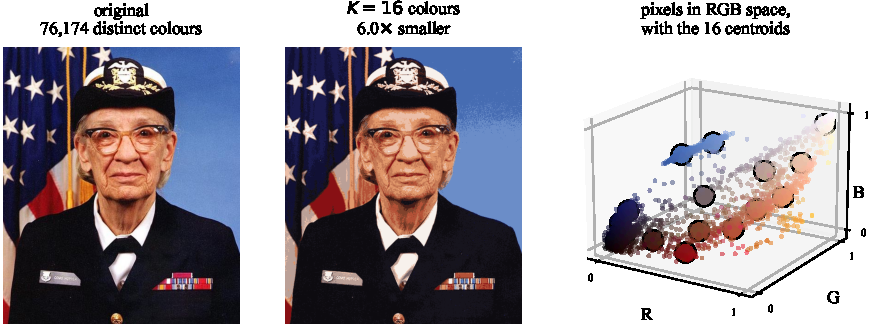
\includegraphics[width=\textwidth]{figs/fig_compression.pdf}
\caption{Colour quantisation by $K$-means, $K = 16$. The photograph contains
76{,}174 distinct colours; the reconstruction uses sixteen and remains clearly
legible, with visible banding in the smooth background where the palette is
too coarse. Right: a subsample of the pixels plotted in RGB space, each drawn
in its own colour, with the sixteen centroids. The clusters are the natural
colour families of the image: skin tones, navy uniform, red and white
flag.}
\label{fig:compression}
\end{figure}

The arithmetic, for the $512 \times 600$ image shown:
\begin{align*}
\text{original} \quad&
  307{,}200 \text{ pixels} \times 24 \text{ bits}
  = 7{,}372{,}800 \text{ bits} ,\\
\text{compressed} \quad&
  \underbrace{307{,}200 \times 4 \text{ bits}}_{\text{one index per pixel}}
  \;+\;
  \underbrace{16 \times 24 \text{ bits}}_{\text{the palette}}
  = 1{,}229{,}184 \text{ bits} ,
\end{align*}
a factor of $6.0$. This is \emph{lossy} compression: the original colours
cannot be recovered, and \eqref{eq:distortion} is precisely the mean squared
reconstruction error you are choosing to accept. Note also the practical
shortcut used here. The centroids were fitted on a random subsample of
8{,}000 pixels rather than all 307{,}200, because the centroid of a colour
family is estimated perfectly well from a sample, and only the final
assignment needs to touch every pixel.

\partline{Part II\quad Anomaly detection by density estimation}{find the
things that do not belong}

\section{Anomaly detection: the algorithm}

Fit a density $p(x)$ to data that is unlabelled and almost entirely normal.
For a new example $x_{\text{test}}$, compute $p(x_{\text{test}})$ and
\begin{equation}
\text{flag } x_{\text{test}} \text{ as anomalous} \iff
p(x_{\text{test}}) < \varepsilon .
\label{eq:rule}
\end{equation}

That is the whole algorithm (Figure~\ref{fig:concept}). The motivating case is
manufacturing: after an aircraft engine comes off the line you measure
features such as heat generated ($x_1$) and vibration intensity ($x_2$). A
manufacturer produces very few bad engines, so collecting normal examples is
easy and collecting defective ones is not. The technique is called
\emph{density estimation}, and the same pattern appears in fraud detection
(login frequency, pages visited, transactions, typing speed), data-centre
monitoring (memory, disk accesses per second, CPU load, and ratios such as CPU
load over network traffic), and telecom cell-tower monitoring.

\begin{figure}[t]
\centering
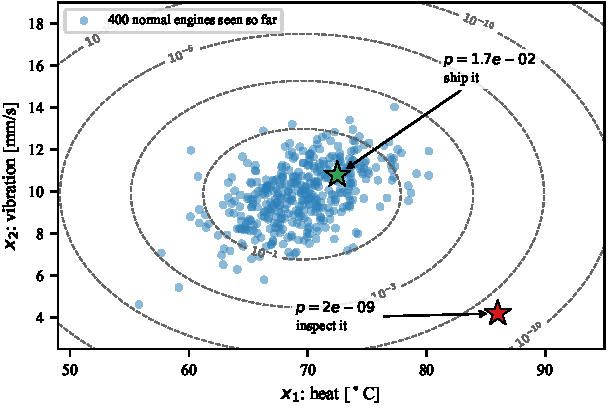
\includegraphics[width=0.66\textwidth]{figs/fig_concept.pdf}
\caption{The decision rule \eqref{eq:rule} on 400 normal engines. Contours are
labelled by how far $p$ has fallen below its peak. The green engine sits where
the training data are dense and is passed; the red one sits where $p$ is seven
orders of magnitude smaller and is sent for inspection. Note that in fraud
detection the response to a flag is \emph{not} to close the account. It is
to escalate: ask the security team to look, request identity verification, or
serve a CAPTCHA. The detector buys attention, not a verdict.}
\label{fig:concept}
\end{figure}

\subsection*{The three steps}

\begin{enumerate}[label=\textbf{\arabic*.}]
\item Choose features $x_j$ that you think might take unusually large or small
      values for an anomalous example.
\item Fit the parameters. For each feature $j = 1,\dots,n$,
      \begin{equation}
      \mu_j = \frac{1}{m}\sum_{i=1}^{m} x_j^{(i)} ,
      \qquad
      \sigma_j^2 = \frac{1}{m}\sum_{i=1}^{m}\bigl(x_j^{(i)} - \mu_j\bigr)^2 .
      \label{eq:fit}
      \end{equation}
\item For a new $x$, compute
      \begin{equation}
      p(x) = \prod_{j=1}^{n} p\bigl(x_j;\mu_j,\sigma_j^2\bigr)
           = \prod_{j=1}^{n} \frac{1}{\sqrt{2\pi}\,\sigma_j}
             \exp\!\left(-\frac{(x_j-\mu_j)^2}{2\sigma_j^2}\right)
      \label{eq:product}
      \end{equation}
      and apply \eqref{eq:rule}.
\end{enumerate}

Two details. The variance in \eqref{eq:fit} is divided by $m$, not $m-1$: this
is the maximum-likelihood estimate, and it is what the graded exercises check.
The difference is a factor $m/(m-1)$, about $0.3\%$ at $m = 307$, and gets
absorbed entirely into the choice of $\varepsilon$.

Second, the product in \eqref{eq:product} assumes the features are
statistically independent. This is essentially always false, and the method
works anyway, but the assumption has a sharp geometric consequence, which
is the subject of Section~\ref{sec:cov}.

\begin{figure}[t]
\centering
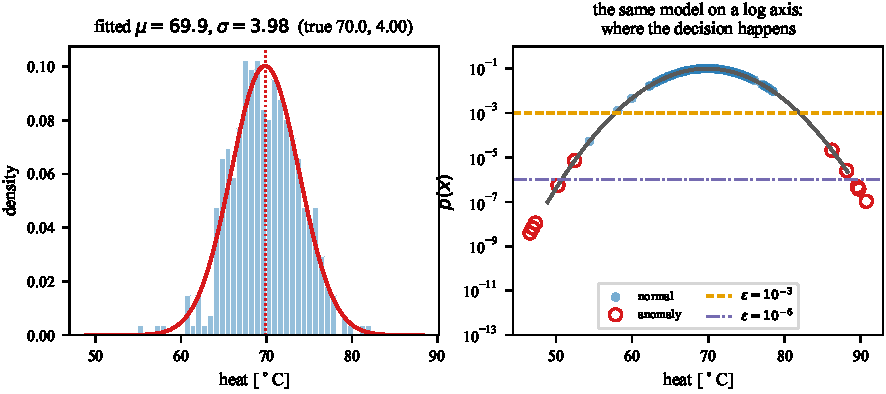
\includegraphics[width=\textwidth]{figs/fig_gaussian1d.pdf}
\caption{A single feature, so the whole model is visible. Left: 400 normal
engines and the density fitted by \eqref{eq:fit}. Right: the same density on a
logarithmic axis, with 160 validation examples scored by it. The left panel is
what the model believes; the right panel is what you make decisions with. On a
linear density axis the entire anomaly region is pinned indistinguishably
against zero, while on a log axis it spreads over ten orders of magnitude,
and every thresholding decision lives in exactly that range.}
\label{fig:gaussian1d}
\end{figure}

\section{Evaluating it, and choosing $\varepsilon$}

You cannot choose $\varepsilon$ from the training data, because it contains no
anomalies: nothing in it indicates where ``too improbable'' begins. So keep
three splits:

\begin{center}\small
\begin{tabular}{@{}lll@{}}
\toprule
split & contents & purpose \\
\midrule
train      & normal only, unlabelled              & fit $\mu_j, \sigma_j^2$ \\
validation & mostly normal $+$ a few labelled anomalies & choose $\varepsilon$ \\
test       & same mixture                          & report the score, \emph{once} \\
\bottomrule
\end{tabular}
\end{center}

\begin{warnbox}{Never use accuracy}
On a validation set that is $7\%$ anomalous, a detector that flags
\emph{nothing} scores $93\%$ accuracy. In real fraud or manufacturing settings
anomalies are $0.1\%$ or less, and the same do-nothing detector scores
$99.9\%$. Accuracy cannot distinguish a working detector from a switched-off
one, so it gives the search for $\varepsilon$ nothing to climb.
\end{warnbox}

Use the confusion matrix instead (Figure~\ref{fig:confusion}), and see
Figure~\ref{fig:tradeoff} for what the sweep over $\varepsilon$ looks like:
\begin{equation}
\text{prec} = \frac{tp}{tp+fp},
\qquad
\text{rec} = \frac{tp}{tp+fn},
\qquad
F_1 = \frac{2\,\text{prec}\cdot\text{rec}}{\text{prec}+\text{rec}} .
\label{eq:f1}
\end{equation}

Note that $tn$ appears nowhere in \eqref{eq:f1}. That is precisely why these
quantities survive severe class imbalance: they refuse to take credit for the
enormous pile of normal examples you correctly ignored.

$F_1$ is the \emph{harmonic} mean, which matters. Precision $1.00$ paired with
recall $0.02$ has arithmetic mean $0.51$, which looks respectable, and $F_1 =
0.039$, which is correctly damning. Any usable metric here must punish that
combination, because ``flag the single most improbable example and nothing
else'' achieves perfect precision while being useless.

\begin{figure}[t]
\centering
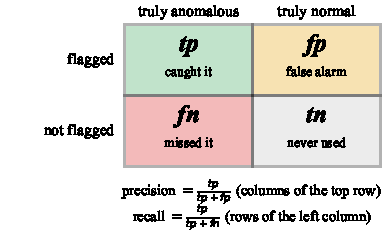
\includegraphics[width=0.52\textwidth]{figs/fig_confusion.pdf}
\caption{The four outcomes of a flagging decision. Only three of the cells
appear in \eqref{eq:f1}: the count of correctly ignored normal examples,
$tn$, is deliberately discarded.}
\label{fig:confusion}
\end{figure}

\begin{figure}[t]
\centering
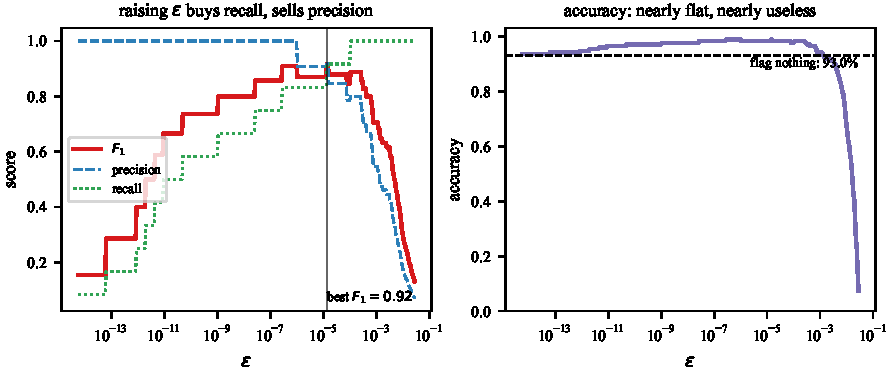
\includegraphics[width=\textwidth]{figs/fig_tradeoff.pdf}
\caption{Sweeping $\varepsilon$ over the full twelve decades spanned by
$p$ on the validation set. As $\varepsilon$ grows the flagged set only ever
grows, so recall rises monotonically and precision falls monotonically; $F_1$
rises, peaks, and falls, and the search finds that peak. Accuracy, meanwhile,
is nearly flat at the base rate across the entire sweep.}
\label{fig:tradeoff}
\end{figure}

\begin{keybox}{$F_1$ is a choice, not a law}
You are picking a point on a trade-off curve, not finding a correct answer.
$F_1$ weights precision and recall equally, which is a specific and often
wrong opinion. For aircraft engines a missed defect costs vastly more than a
needless inspection, so the better objective is to maximise recall subject to
a false-alarm budget you can actually staff, say twenty inspections a day.
That formulation also needs no labels, which is often decisive.
\end{keybox}

\section{Anomaly detection versus supervised learning}

Both can be pointed at the same labelled data, so the choice needs a
criterion. It is not simply how many positives you have; it is what \emph{kind}
of positives to expect next.

\begin{center}\small
\begin{tabular}{@{}p{0.46\textwidth}p{0.46\textwidth}@{}}
\toprule
\textbf{Use anomaly detection} & \textbf{Use supervised learning} \\
\midrule
Very few positive examples (0--20 is typical); many negatives. &
Plenty of both positive and negative examples. \\[3pt]
Many \emph{different} kinds of anomaly, and the next one may look nothing
like anything you have seen. &
Future positives are likely to resemble the positives in your training set. \\[3pt]
\emph{Examples}: fraud, manufacturing defects, machine and infrastructure
failures. &
\emph{Examples}: spam filtering, weather prediction, disease classification. \\
\bottomrule
\end{tabular}
\end{center}

The logic: if the algorithm cannot learn what a positive looks like from
examples, because the next defect will be a genuinely new kind of defect,
then do not try. Model normality instead, and flag departure from it. A
supervised classifier trained on the defects you happened to see will
confidently pass a defect of a kind it has never met; a density model will not.

\section{Feature engineering beats model choice}
\label{sec:features}

\subsection*{Make each feature roughly Gaussian}

Histogram every feature before modelling it. If one is skewed, transform it:
$\log x$, $\log(x+c)$, $\sqrt{x}$, $x^{0.3}$ are the usual candidates. Apply
the \emph{same} transform to the training, validation and test sets.

Figure~\ref{fig:numerics}(a) shows why this is not cosmetic. The feature is a
log-normal latency, and it carries \textbf{no anomaly signal whatsoever}.
Anomalous servers in this dataset were drawn from exactly the same latency
distribution as healthy ones; the signal lives entirely in a second,
well-behaved feature. Fitting a Gaussian to it directly inflates the variance
to cover the legitimate right tail, which places $11\%$ of the model's
probability mass on \emph{negative} latency. Honest slow-but-fine servers then
land four standard deviations out and outrank the genuinely broken ones.

\begin{center}\small
\begin{tabular}{@{}lcccc@{}}
\toprule
features & validation $F_1$ & precision & recall & test $F_1$ \\
\midrule
latency as given & 0.750 & 0.609 & 0.933 & 0.737 \\
$\log(\text{latency})$ & 1.000 & \textbf{1.000} & 0.933 & \textbf{0.966} \\
\bottomrule
\end{tabular}
\end{center}

Recall is untouched; precision moves from $0.609$ to $1.000$. \textbf{Bad
feature shape costs you precision, not recall}, and a detector that cries
wolf gets switched off, which is operationally identical to not having one.

\subsection*{Error analysis, and combination features}

When an anomaly slips through with a large $p(x)$, look at that example and
ask what new feature would have distinguished it. Often the answer is a
\emph{ratio} or product of existing features: neither CPU load nor network
traffic is individually unusual, but their ratio is. Adding CPU/network as its
own column lets the product model \eqref{eq:product} express a relationship it
otherwise structurally cannot.

\begin{figure}[t]
\centering
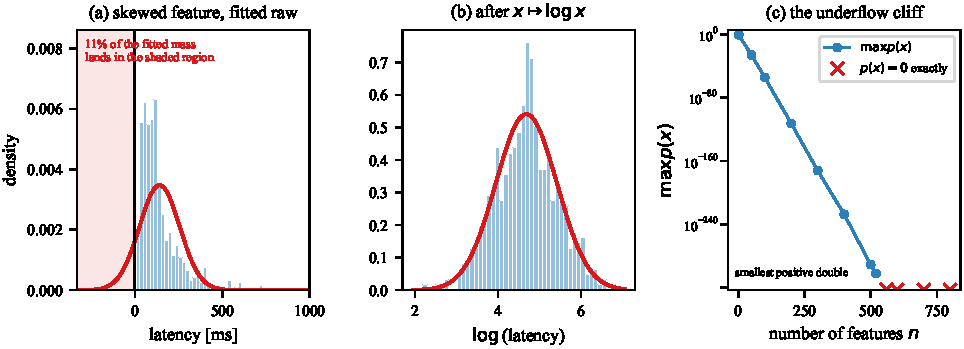
\includegraphics[width=\textwidth]{figs/fig_numerics.pdf}
\caption{(a) A Gaussian fitted to a log-normal feature: the mean is dragged
above the mode, the variance inflates to cover the tail, and $11\%$ of the
fitted mass falls on physically impossible negative values. (b) The same
feature after $x \mapsto \log x$; the skewness drops from $2.24$ to $-0.02$.
(c) The product \eqref{eq:product} decays like $e^{-1.42n}$ for standard
normal data and reaches the smallest positive double near $n = 520$. Beyond
that, $p(x)$ is exactly $0.0$ for every example.}
\label{fig:numerics}
\end{figure}

\begin{warnbox}{Work in $\log p$, not $p$}
Figure~\ref{fig:numerics}(c) is a failure with no statistical content at all.
Once $n$ exceeds roughly $520$, every $p(x)$ underflows to exactly $0.0$, so
$p(x) < \varepsilon$ is true for \emph{everything} and the detector flags
$100\%$ of your data, while looking like a badly tuned threshold rather than
an arithmetic problem. Evaluate
\[
\log p(x) = -\frac{1}{2}\sum_{j=1}^{n}
  \left[ \frac{(x_j-\mu_j)^2}{\sigma_j^2} + \log \sigma_j^2
         + \log 2\pi \right]
\]
instead, and the failure mode does not exist: a sum of logs has no cliff. For
the same reason, space the search grid for $\varepsilon$ uniformly in $\log p$
rather than in $p$. A grid uniform in $p$ places nearly all of its nodes in
the top decade, where nothing is being decided, and resolves the tail with one
or two points.
\end{warnbox}

\section{What the independence assumption costs}
\label{sec:cov}

Because \eqref{eq:product} is a product of per-feature densities, its level
sets are \textbf{axis-aligned ellipses}. The model can therefore only ever
notice ``this one coordinate is extreme''. An example that is perfectly
ordinary in \emph{every individual feature} while being impossible as a
\emph{combination} is invisible to it.

Figure~\ref{fig:cov} is built to make this quantitative. The data have
correlation $0.93$, and the anomalies were chosen so that every one of them
lies within $2.1$ standard deviations of the mean in \emph{every} coordinate,
while the most extreme \emph{normal} point reaches $2.63$. Marginally, then,
the anomalies are \emph{less} extreme than ordinary data, and no per-feature
rule, whether a $z$-score cut, a bounding box or a product of marginals, can
separate them at any threshold.

\begin{figure}[t]
\centering
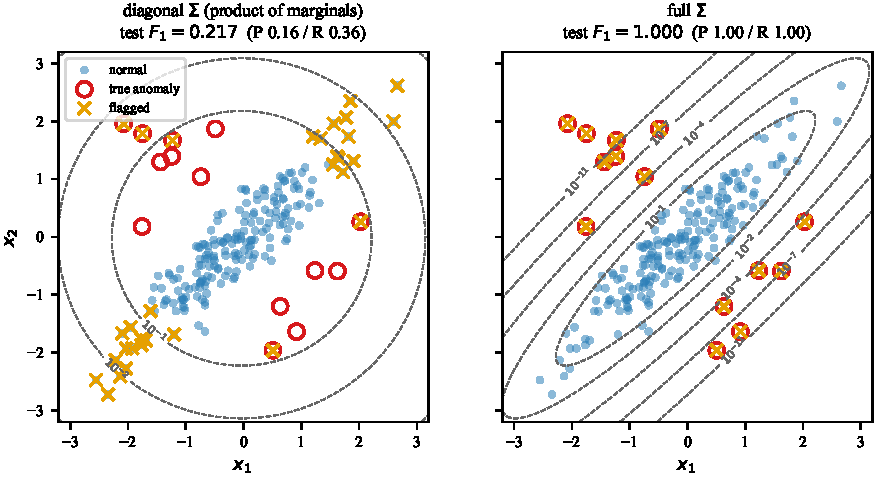
\includegraphics[width=\textwidth]{figs/fig_covariance.pdf}
\caption{Identical data, identical machinery; the only difference is whether
$\Sigma$ may have off-diagonal entries. Left: the diagonal model's contours are
nearly circular, they swallow the anomalies whole, and the threshold that best
fits the validation set flags normal points at the corners instead. Right: the
full-covariance contours follow the ridge and every anomaly falls outside them.
Test $F_1$ goes from $0.217$ to $1.000$.}
\label{fig:cov}
\end{figure}

The fix is the \textbf{multivariate Gaussian}, which replaces the $n$ separate
variances by a full covariance matrix:
\begin{equation}
p(x;\mu,\Sigma) = \frac{1}{(2\pi)^{n/2}\,|\Sigma|^{1/2}}
  \exp\!\left(-\tfrac12 (x-\mu)^{\!\top}\Sigma^{-1}(x-\mu)\right),
\qquad
\Sigma = \frac{1}{m}\sum_{i=1}^m (x^{(i)}\!-\mu)(x^{(i)}\!-\mu)^{\!\top}.
\label{eq:mvn}
\end{equation}
Its contours can tilt, so correlations are captured automatically. The original
model \eqref{eq:product} is exactly \eqref{eq:mvn} with $\Sigma$ constrained to
be diagonal.

\begin{center}\small
\begin{tabular}{@{}lll@{}}
\toprule
 & independent (product) & multivariate Gaussian \\
\midrule
parameters & $2n$ & $n + n(n+1)/2$ \\
correlations & only via hand-built features & automatic \\
data needed & works at $m \approx n$ & needs $m > 10n$; $\Sigma$ singular if $m < n$ \\
cost & $O(n)$ per example & $O(n^3)$ once, $O(n^2)$ per example \\
\bottomrule
\end{tabular}
\end{center}

\begin{keybox}{Computing the multivariate density properly}
Do not form $\Sigma^{-1}$ or $|\Sigma|$. Take the Cholesky factor
$\Sigma = LL^{\!\top}$ once; then solving $Lw = x-\mu$ gives
$w^{\!\top}w = (x-\mu)^{\!\top}\Sigma^{-1}(x-\mu)$, and
$\log|\Sigma| = 2\sum_i \log L_{ii}$ comes free. One factorisation, no
explicit inverse, no overflow in the determinant, and better conditioning.
\end{keybox}

\section{A worked case: the two fixes are not independent}

To close, a six-feature problem where both of the preceding sections are
needed at once. The data are telemetry from an iterative linear solver:
estimated condition number, iteration count, final residual, residual decay
rate, preconditioner setup time, peak memory. Problem size and conditioning
are \emph{latent} rather than columns, so they induce genuine correlation
between the columns you do observe. Three failure modes are planted:
stagnation at the iteration cap; preconditioner degradation, where a run needs
about twice the iterations its conditioning predicts; and a silently easier
problem, where the operator came out far better conditioned than the mesh
warrants. Recall is reported per mode, because the aggregate hides everything:
each mode is only $8$ of $424$ examples.

\begin{center}\small
\begin{tabular}{@{}lcccc@{}}
\toprule
model & test $F_1$ & \multicolumn{3}{c}{recall by failure mode} \\
\cmidrule(l){3-5}
 & & stagnation & precond.\ degrad. & easier problem \\
\midrule
raw $+$ diagonal $\Sigma$            & 0.345 & 0.62 & 0.00 & 0.00 \\
raw $+$ full $\Sigma$                & 0.345 & 0.62 & 0.00 & 0.00 \\
$\log$ $+$ diagonal $\Sigma$         & 0.744 & 1.00 & 0.00 & 1.00 \\
$\log$ $+$ full $\Sigma$             & \textbf{0.958} & 1.00 & 1.00 & 0.88 \\
$\log$ $+$ residual feature $+$ diagonal $\Sigma$ & 0.941 & 1.00 & 1.00 & \textbf{1.00} \\
\bottomrule
\end{tabular}
\end{center}

The first two rows are the point. Giving the model a full covariance matrix on
the raw features buys \textbf{exactly nothing}. The real dependence here is
\[
\texttt{iters} \;\approx\; a + b\,\log_{10}(\texttt{cond}) + \text{noise},
\]
which is not linear in the raw coordinates: the raw correlation between
\texttt{cond} and \texttt{iters} is $+0.430$, and after the transform it is
$+0.876$. Covariance can only capture \emph{linear} structure, so the
transform is a \emph{precondition} for the covariance model, not an
alternative to it. The two fixes are not independent improvements between
which one chooses.

The last row is the other lesson. Regressing \texttt{iters} on
$\log_{10}(\texttt{cond})$ on the training set and supplying the residual as a
single extra feature hands the \emph{cheap diagonal} model the same
conditional information the full covariance had to discover, and reaches
perfect recall on all three modes with $O(n)$ parameters instead of $O(n^2)$.
It also produces something you can hand to whoever gets paged: \emph{this run
took 2.1 times the iterations its conditioning predicts}. Reach for a richer
model when you cannot name the structure; when you can name it, build the
feature.

\begin{keybox}{Where the two parts meet}
The single Gaussian of \eqref{eq:product} assumes normality has \emph{one}
centre. If your normal data are genuinely multimodal (two populations of
machine, or daytime and overnight traffic), the fitted Gaussian puts its peak
in the empty space \emph{between} the modes and assigns low density to both,
so it flags healthy examples from each. The repair is Part~I: cluster the
training data first, then either fit one density per cluster, or use the
distance to the nearest centroid in place of $p(x)$. Clustering finds where
the data are; density estimation says how surprised to be at a new point.
They compose.
\end{keybox}

\begin{keybox}{If you remember seven things}
\begin{enumerate}[label=\arabic*.,leftmargin=*]
\item \textbf{($K$-means)} Assign to the nearest centroid, move each centroid
      to the mean of its own points. Both steps minimise the same distortion
      $J$. It must therefore never increase, which is your best debugging
      check.
\item \textbf{($K$-means)} Convergence is to a \emph{local} optimum. Restart
      from many random data points and keep the lowest $J$; here seven runs in
      forty got stuck at four times the best value.
\item \textbf{($K$-means)} $J$ falls monotonically with $K$, so it can never
      choose $K$ for you. The elbow is often absent. Choose $K$ by what the
      clusters are for.
\item Fit $p(x)$ on normal data, flag when $p(x) < \varepsilon$. That is the
      entire anomaly-detection algorithm.
\item Tune $\varepsilon$ on a small labelled validation set using $F_1$ or a
      false-alarm budget, never accuracy.
\item Use anomaly detection when future anomalies will not resemble past ones;
      use supervised learning when they will.
\item Histogram every feature and transform the skewed ones; this buys more
      than any change of model. And remember the product form assumes
      independence, which forces axis-aligned contours. Fix that with
      engineered combination features or a full covariance matrix, transforming
      first, because covariance sees only linear structure.
\end{enumerate}
\end{keybox}

\bigskip
\noindent\small\textit{Every figure and table in these notes was produced by
running the algorithms on the stated datasets. The implementations are in}
\texttt{kmeans/} \textit{and} \texttt{anomaly-detection/} \textit{in this
repository; the figures are generated by} \texttt{notes/make\_figs.py}\textit{.}

\end{document}
